\documentclass[a4paper]{article}
\usepackage{amsmath,amssymb,algorithmic,booktabs,bm,caption,cases,clrscode3e,csvsimple,enumerate,float,geometry,graphicx,indentfirst,makecell,multirow,setspace,tabularx,titlesec}
\captionsetup[figure]{labelsep=period}
\captionsetup[table]{labelsep=period}
\geometry{left=3.5cm,right=3.5cm,top=3.3cm,bottom=3.3cm}
\renewcommand\thesection{\arabic{section}}
\setlength{\parindent}{2em}
\begin{document}
\begin{center}
\huge
\textbf{VE216\\Introduction to Signals and Systems\\}
\Large
\vspace{30pt}
\uppercase{Homework 3 Attached Pages}\\
\vspace{5pt}\today\\
\vspace{5pt}
Yihua Liu 518021910998
\vspace{5pt}
\rule[-10pt]{.97\linewidth}{0.05em}
\end{center}

6. The Fourier series representation of 4(a) is
\begin{figure}[H]
    \begin{center}
        \includegraphics[width=0.6\textwidth]{6-1.eps}
    \end{center}
    \caption{6-1.}
\end{figure}

The Fourier series representation of 4(b) is
\begin{figure}[H]
    \begin{center}
        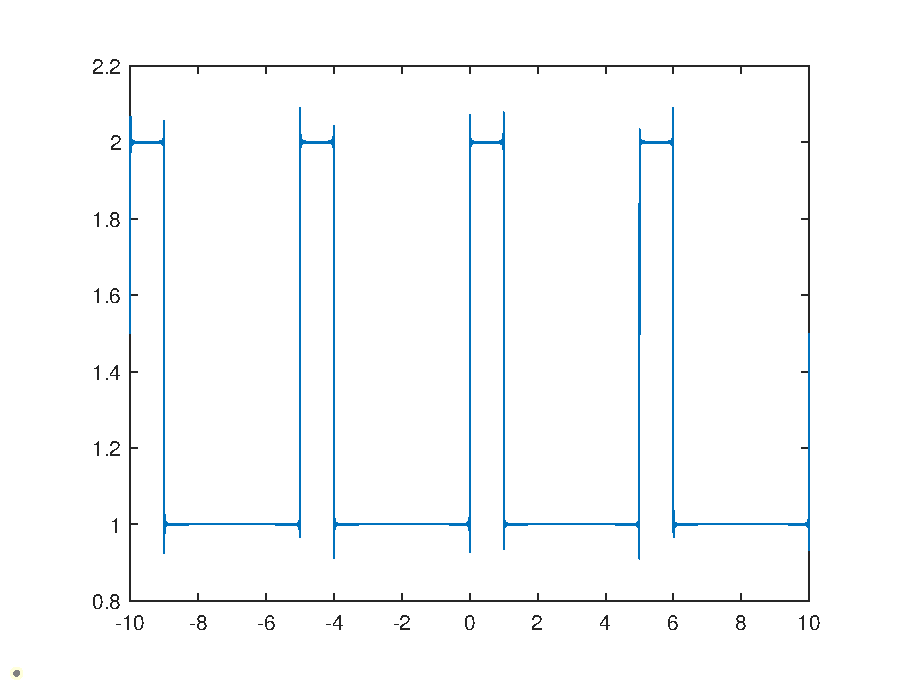
\includegraphics[width=0.6\textwidth]{6-2.eps}
    \end{center}
    \caption{6-2.}
\end{figure}

The Fourier series representation of 4(c) is
\begin{figure}[H]
    \begin{center}
        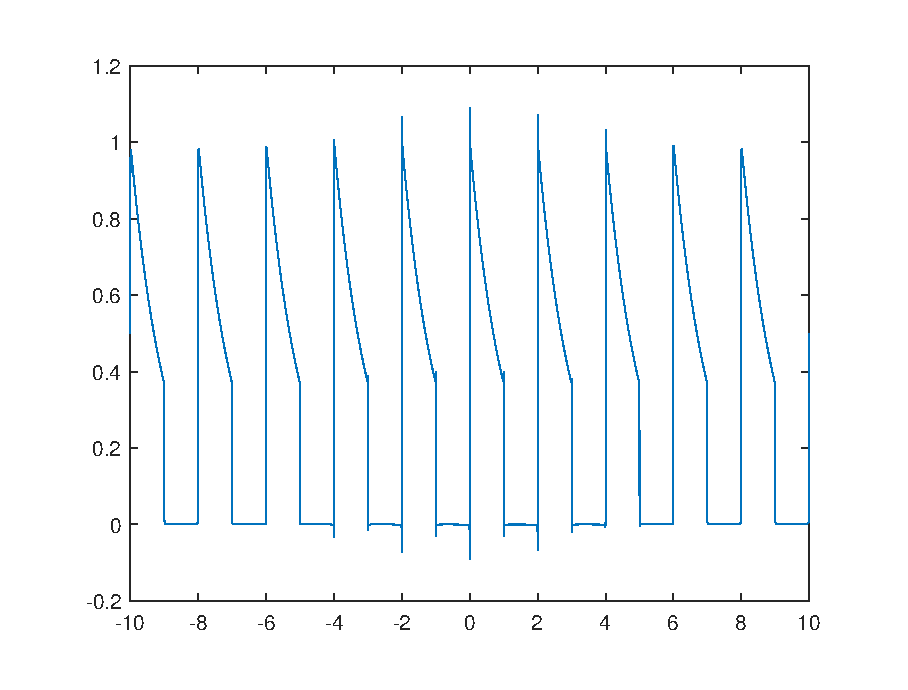
\includegraphics[width=0.6\textwidth]{6-3.eps}
    \end{center}
    \caption{6-3.}
\end{figure}

8.

(a) The graph of $S_N(t)$ with $N=5$ for $t\in[0.5,4.5]$ is
\begin{figure}[H]
    \begin{center}
        \includegraphics[width=0.6\textwidth]{8(a)-1.eps}
    \end{center}
    \caption{8(a)-1.}
\end{figure}

The graph of $S_N(t)$ with $N=10$ for $t\in[0.5,4.5]$ is
\begin{figure}[H]
    \begin{center}
        \includegraphics[width=0.6\textwidth]{8(a)-2.eps}
    \end{center}
    \caption{8(a)-2.}
\end{figure}

The graph of $S_N(t)$ with $N=15$ for $t\in[0.5,4.5]$ is
\begin{figure}[H]
    \begin{center}
        \includegraphics[width=0.6\textwidth]{8(a)-3.eps}
    \end{center}
    \caption{8(a)-3.}
\end{figure}

The graph of $S_N(t)$ with $N=19$ for $t\in[0.5,4.5]$ is
\begin{figure}[H]
    \begin{center}
        \includegraphics[width=0.6\textwidth]{8(a)-4.eps}
    \end{center}
    \caption{8(a)-4.}
\end{figure}

From the graphs I see that the general shape and discontinuities of $S_N(t)$ does not change obviously as $N$ increases, but the sawteeth of the curve increases as $N$ increases proportionally. In general, the shape of the graph becomes closer to $x(t)$ as $N$ increases.

(b) Use Matlab to calculate $S_N(0)$ and $S_N(1)$ for the N values in (a).

When $N=5$, $S_N(0)=0.4822$, $S_N(1)=0.1891$.

When $N=10$, $S_N(0)=0.4902$, $S_N(1)=0.1879$.

When $N=15$, $S_N(0)=0.4935$, $S_N(1)=0.1861$.

When $N=19$, $S_N(0)=0.4949$, $S_N(1)=0.1857$.

Hence, we can make an educated guess that $S_N(0)\rightarrow\frac{1}{2}$ and $S_N(1)\rightarrow\frac{1}{2e}$ when $N\rightarrow\infty$.

10.

(d) The graph of the magnitude of the system's frequency response $|H(j\omega)|$ as a function of $\omega$ is
\begin{figure}[H]
    \begin{center}
        \includegraphics[width=0.6\textwidth]{10(d).eps}
    \end{center}
    \caption{10(d).}
\end{figure}

(e) The MATLAB code is shown below:
\begin{codebox}
    \li a=[1];
    \li b=[1 1 1];
    \li w=linspace(-5,5,10000);
    \li h=freqs(a,b,w);
    \li plot(w,abs(h));
\end{codebox}

The graph is
\begin{figure}[H]
    \begin{center}
        \includegraphics[width=0.6\textwidth]{10(e).eps}
    \end{center}
    \caption{10(e).}
\end{figure}

(f) The power density spectrum of $x(t)$ is
\begin{figure}[H]
    \begin{center}
        \includegraphics[width=0.6\textwidth]{10(f).eps}
    \end{center}
    \caption{10(f).}
\end{figure}

(h) The power density spectrum of $y(t)$ is
\begin{figure}[H]
    \begin{center}
        \includegraphics[width=0.6\textwidth]{10(h).eps}
    \end{center}
    \caption{10(h).}
\end{figure}

12.

(a) The graph of the filter's magnitude response is
\begin{figure}[H]
    \begin{center}
        \includegraphics[width=0.6\textwidth]{12(a).eps}
    \end{center}
    \caption{12(a).}
\end{figure}

(b) The graph of the generated signal is
\begin{figure}[H]
    \begin{center}
        \includegraphics[width=0.6\textwidth]{12(b).eps}
    \end{center}
    \caption{12(b).}
\end{figure}

(c) The graph of the output signal is
\begin{figure}[H]
    \begin{center}
        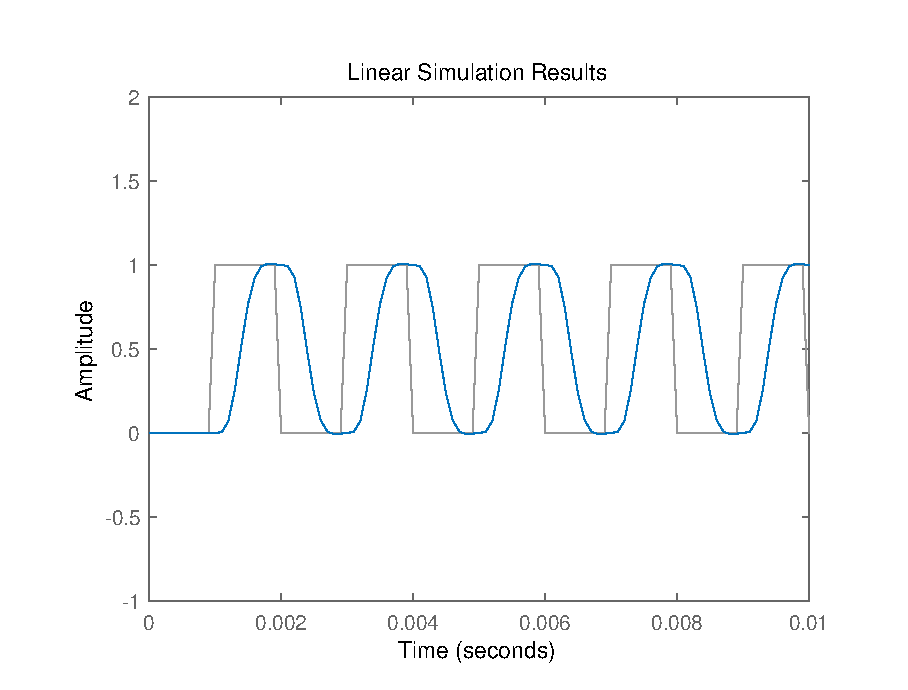
\includegraphics[width=0.6\textwidth]{12(c).eps}
    \end{center}
    \caption{12(c).}
\end{figure}
\end{document}